\documentclass[a4paper,leqno,nobib,sfsidenotes]{tufte-book}


%% Paquetes relacionados con el lenguaje y la localización del texto
\usepackage[utf8]{inputenc}
\usepackage[T1]{fontenc}
\usepackage[spanish,es-tabla]{babel}
\usepackage{csquotes}   %% Comillas dobles
\decimalpoint           %% Usar punto decimal en lugar de una coma
\usepackage[
  backend=biber,
  natbib=true,
  autocite=footnote,    %% Inserta las ref. en el margen con \autocite
  style=authoryear,     %% Orden en que aparece la info. en la bibliografía
  uniquename=init,      %% Usa iniciales para distinguir apellidos repetidos
  maxcitenames=2,       %% Se citan a lo más dos autores
  mincitenames=1,
  doi=false,            %% Ignora estos campos del archivo .bib
  isbn=false,
  url=false,
  eprint=false,
  dashed=false
]{biblatex}


%% Paquetes relacionados con tablas, figuras y otras gráficas
\usepackage{float}      %% Para gráficos flotantes en la página
\usepackage{booktabs}   %% Para tablas más sofisticadas
\usepackage{multirow}   %% Para columnas y renglones extendidos en tablas
\usepackage{graphicx}   %% Para gráficos generales


%% Paquetes relacionados con el formato de ciertas secciones del texto
\usepackage{caption}    %% Para el texto debajo de gráficos flotantes
\usepackage{multicol}   %% Para secciones con texto dividido en columnas
\usepackage{enumitem}   %% Para listas con viñetas
\setlist[itemize]{label=\textbullet}


%% Paquetes relacionados con los ambientes matemáticos
\usepackage{amsmath}
\usepackage{amsthm}
\usepackage{amssymb}

%% Definición de los ambientes matemáticos
\providecommand{\casename}{Caso}
\providecommand{\definitionname}{Definición}
\providecommand{\examplename}{Ejemplo}
\providecommand{\propositionname}{Proposición}
\providecommand{\theoremname}{Teorema}
\providecommand{\lemmaname}{Lema}
\providecommand{\corollaryname}{Corolario}
\providecommand{\remarkname}{Escolio}
\theoremstyle{definition}
\newtheorem{defn}{\protect\definitionname}
\newtheorem{expl}{\protect\examplename}
\theoremstyle{plain}
\newtheorem{prop}{\protect\propositionname}
\newtheorem{thm}{\protect\theoremname}
\newtheorem{lem}{\protect\lemmaname}
\newtheorem{cor}{\protect\corollaryname}
\theoremstyle{remark}
\newtheorem{rem}{\protect\remarkname}

%% Configuración del enumerado de los ambientes matemáticos
\newlist{casenv}{enumerate}{4}
\setlist[casenv]{leftmargin=*,align=left,widest={iiii}}
\setlist[casenv,1]{label={{\itshape\ \casename} \arabic*.},ref=\arabic*}
\setlist[casenv,2]{label={{\itshape\ \casename} \roman*.},ref=\roman*}
\setlist[casenv,3]{label={{\itshape\ \casename\ \alph*.}},ref=\alph*}
\setlist[casenv,4]{label={{\itshape\ \casename} \arabic*.},ref=\arabic*}

%% Símbolo para indicar el final de un ejemplo
\newcommand\xqed[1]{\leavevmode\unskip\penalty9999 \hbox{}\nobreak\hfill\quad\hbox{#1}}
\newcommand\exend{\xqed{\(\blacklozenge\)}}


%% Configuración para colocar automáticamente hipervínculos en el PDF
\PassOptionsToPackage{
  unicode=true,
  pdfusetitle,
  bookmarks=true,
  bookmarksnumbered=true,
  bookmarksopen=false,
  breaklinks=false,
  pdfborder={0 0 1},
  backref=false,
  colorlinks=false
}{hyperref}


%% Configuración para escribir pseudocódigo
\usepackage[vlined,linesnumbered,ruled]{algorithm2e}
\setkeys{Gin}{width=\linewidth,totalheight=\textheight,keepaspectratio}

\SetKw{Error}{error}
\SetKw{And}{and}
\SetKw{Or}{or}
\SetKw{Not}{not}
\SetKw{True}{true}
\SetKw{False}{false}
\SetKw{Nil}{nil}
\SetKw{Down}{down to}
\SetCommentSty{textit}
\SetKwComment{Comment}{$\triangleright$ }{}
\SetFuncSty{textsc}
\DontPrintSemicolon
\SetAlgorithmName{Pseudocódigo}{}


%% Se eliminan algunos campos innecesarios de las ref. bibliográficas
\makeatletter
\AtBeginDocument{
  \AtEveryBibitem{\clearfield{month}}
  \AtEveryBibitem{\clearfield{day}}
  \AtEveryBibitem{\clearfield{note}}
  \AtEveryBibitem{\clearlist{location}}
  \AtEveryBibitem{\clearfield{eventtitle}}
  \DeclareFieldFormat[article,inbook,incollection,inproceedings,patent,thesis,unpublished]{citetitle}{#1}
  \DeclareFieldFormat[article,inbook,incollection,inproceedings,patent,thesis,unpublished]{title}{#1} 
}
\makeatother


\title{Apuntes sobre computación}
\author{Carlos A. Oliva Moreno}
\addbibresource{referencias.bib}

\begin{document}
  \maketitle
  
  \tableofcontents{}
  
  \part{Matemáticas discretas}
    \chapter{Lógica formal}

\section{Los conectores lógicos}

Sean \(P\) y \(Q\) dos proposiciones.

\begin{table}[h]
  \caption{%
    La tabla de verdad que define formalmente cada uno de los conectores lógicos básicos que se explican aquí.
  }
  \label{tab:logical_connectors}
  \begin{centering}
    \begin{tabular}{c c c c c c c}
      \toprule
        \(P\) & \(Q\) & \(\neg P\) & \(P\land Q\) & \(P\lor Q\) & \(P\to Q\) & 
        \(P\leftrightarrow Q\) \\
      \midrule
        \(T\) & \(T\) & \(F\) & \(T\) & \(T\) & \(T\) & \(T\) \\
        \(T\) & \(F\) & & \(F\) & \(T\) & \(F\) & \(F\) \\
        \(F\) & \(T\) & \(T\) & \(F\) & \(T\) & \(T\) & \(F\) \\
        \(F\) & \(F\) & & \(F\) & \(F\) & \(T\) & \(T\) \\
      \bottomrule
    \end{tabular}
  \par\end{centering}
\end{table}

\marginnote[1.5\baselineskip]{%
  La hipótesis y conclusión también se conocen como \textbf{antecedente} y \textbf{consecuente} y como \textbf{hipótesis} y \textbf{tesis}, respectivamente. 
  Así mismo, la recíproca y la contrarecíproca también se conocen como el \textbf{converso} y el \textbf{inverso}, respectivamente.
  Por otro lado, la condicional vacíamente verdadera también se denomina \textbf{verdadera por defecto}.
}

Dada una proposición \(P\to Q\):
\begin{itemize}
  \item La \textbf{hipótesis} es \(P\).
  \item La \textbf{conclusión} es \(Q\).
  \item La \textbf{recíproca} es \(Q\to P\).
  \item La \textbf{contrarecíproca} es \(\neg P\to\neg Q\).
  \item La condicional \textbf{no} es conmutativa; \(P\to Q\) \textbf{no} es lo mismo que \(Q\to P\).
  \item Se dice que una condicional es \textbf{vacíamente verdadera} cuando es verdadera debido a que la hipótesis es falsa.
\end{itemize}


\section{La tautología y la contradicción}

Para demostrar que una proposición compuesta determinada es una tautología o una contradicción, se construye su tabla de verdad y se verifica que todos los renglones tengan el mismo valor de verdad; esto es, todos sean verdaderos (para la tautología) o todos falsos (para la contradicción).
\newpage


\section{La implicación lógica}

Hay varias formas de demostrar que \(A\Rightarrow B\):
\begin{itemize}
  \item Demostrar que la proposición \(A\to B\) es una tautología, por medio de su tabla de verdad.
  \item Construir las tablas de verdad de \(A\) y \(B\) y verificar que, en cada renglón donde \(A\) es verdadero, \(B\) también lo sea.
  \item Suponer que \(A\) es verdadero y demostrar que eso conlleva a que \(B\) también lo sea.
  \item Partiendo de \(A\), usar las \emph{reglas de inferencia} para llegar hasta \(B\).
\end{itemize}



\section {La equivalencia lógica}

Hay varias formas de demostrar que \(A\Leftrightarrow B\):
\begin{itemize}
  \item Demostrar que la proposición \(A\leftrightarrow B\) es una tautología, por medio de su tabla de verdad.
  \item Construir las tablas de verdad de \(A\) y \(B\) y verificar que, en cada renglón, ambas tablas tienen exactamente el mismo valor de verdad.
  \item Suponer que \(A\) es verdadero y demostrar que eso conlleva a que \(B\) también lo sea.
  Luego, suponer que \(B\) es verdadero y demostrar que eso conlleva que \(A\) también lo sea.
  \item Partiendo de \(A\) o de \(B\), usar las \emph{equivalencias lógicas básicas} para llegar hasta \(B\) o \(A\), respectivamente.
\end{itemize}
\newpage



\section{Equivalencias lógicas básicas}

Sean \(P,Q,R\) y \(S\) proposiciones y sea \(\theta\) una tautología y \(\varphi\) una contradicción.
\begin{multicols}{2}
  \emph{Leyes de identidad}
  \[
    \begin{aligned}
      P &\Leftrightarrow P \\
      P\land\theta &\Leftrightarrow P \\
      P\lor\varphi &\Leftrightarrow P
    \end{aligned}
  \]
  \emph{Leyes de indepotencia}
  \[
    \begin{aligned}
      P\land P &\Leftrightarrow P \\
      P\lor P &\Leftrightarrow P
    \end{aligned}
  \]
  \emph{Conmutatividad}
  \[
    \begin{aligned}
      P\land Q &\Leftrightarrow Q\land P \\
      P\lor Q &\Leftrightarrow Q\lor P \\
      P\leftrightarrow Q &\Leftrightarrow Q\leftrightarrow P
    \end{aligned}
  \]
  \emph{Asociatividad}
  \[
    \begin{aligned}
      (P\land Q)\land R &\Leftrightarrow P\land(Q\land R) \\
      (P\lor Q)\lor R &\Leftrightarrow P\lor(Q\lor R)
    \end{aligned}
  \]
  \emph{Distributividad}
  \[
    \begin{aligned}
      P\land(Q\lor R) &\Leftrightarrow (P\land Q)\lor(P\land R) \\
      P\lor(Q\land R) &\Leftrightarrow (P\lor Q)\land(P\lor R)
    \end{aligned}
  \]
  \emph{Leyes de negación}
  \[
    \begin{aligned}
      \neg\theta &\Leftrightarrow \varphi \\
      \neg\varphi &\Leftrightarrow \theta \\
      P\land\neg P &\Leftrightarrow \varphi \\
      P\lor\neg P &\Leftrightarrow \theta
    \end{aligned}
  \]
  \emph{Doble negación}
  \[
    \neg\neg P \Leftrightarrow P
  \]
  \emph{Leyes de DeMorgan}
  \[
    \begin{aligned}
      \neg(P\land Q) &\Leftrightarrow \neg P\lor\neg Q \\
      \neg(P\lor Q) &\Leftrightarrow \neg P\land\neg Q
    \end{aligned}
  \]
  \emph{Leyes de absorción}
  \[
    \begin{aligned}
      P\land(P\lor Q) &\Leftrightarrow P \\
      P\lor(P\land Q) &\Leftrightarrow P
    \end{aligned}
  \]
  \emph{División en casos}
  \[
    (P\lor Q)\to R \Leftrightarrow (P\to R)\land(Q\to R) 
  \]
  \emph{Condicional-Disyuntiva}
  \[
    P\to Q \Leftrightarrow \neg P\lor Q
  \]
  \emph{Negación de la condicional}
  \[
    \neg(P\to Q) \Leftrightarrow P\land\neg Q
  \]
  \emph{Contrapositiva}
  \[
    P\to Q\Leftrightarrow\neg Q\to\neg P
  \]
  \emph{Recíproca-Contrarecíproca}
  \[
    Q\to P \Leftrightarrow \neg P\to\neg Q
  \]
  \emph{Bicondicional-Condicional}
  \[
    P\leftrightarrow Q \Leftrightarrow (P\to Q)\land(Q\to P)
  \]
  \emph{Negación de la bicondicional}
  \[
    \neg(P\leftrightarrow Q)\Leftrightarrow (P\land\neg Q)\lor(Q\land\neg P)
  \]
  \emph{Leyes de la cota universal}
  \[
    \begin{aligned}
      P\land\varphi &\Leftrightarrow\varphi \\
      P\lor\theta &\Leftrightarrow\theta
    \end{aligned}
  \]
\end{multicols}
\marginnote[-1.5\baselineskip]{%
  \textbf{Literatura consultada}: \textcite{bloch_2011} pp. 3-12 y 15-22; \textcite{epp_2004} pp. 1-15 y 17-25
}


  \part{Análisis de algoritmos}
    \chapter{Análisis de la corrección de un algoritmo}

El primer paso al analizar un algoritmo es determinar si este es correcto o incorrecto. 
El procedimiento que se sigue para llevar a cabo esta tarea se denomina \textbf{análisis de la corrección de un algoritmo}.

\section{El contraejemplo}

\marginnote[0.5\baselineskip]{Se recomienda buscar un contraejemplo para un algoritmo antes de hacer la demostración de su corrección.}

\marginnote[1.5\baselineskip]{Si no se encuentra un contraejemplo para un algoritmo determinado, esto no implica que dicho algoritmo es correcto.}

\marginnote[1.5\baselineskip]{La demostración de la corrección de un algoritmo debe explicar no solo por qué el algoritmo es correcto, sino también por qué no es incorrecto.}

Para demostrar que un algoritmo determinado es incorrecto, basta con producir un \textbf{contraejemplo}; esto es, un caso específico para el cual el algoritmo no termina su ejecución o no produce un resultado que cumple las características de salida del problema. 
Para encontrar un contraejemplo, se recomienda experimentar primero con los casos específicos más complicados para el algoritmo; p. ej., aquellos que contengan valores empatados o que mezclen valores de frontera de extremos opuestos. 
El contraejemplo debe ser lo más simple y pequeño posible; idealmente la razón de por qué el algoritmo es incorrecto debe ser inmediatamente clara. 
Así, una vez encontrado un contraejemplo, se recomienda simplificarlo tanto como sea posible y presentarlo junto con el resultado incorrecto que produjo el algoritmo y el resultado correcto que debió producir.

\section{La invariante de lazo}

\marginnote[0.5\baselineskip]{%
  La diferencia entre la invariante de lazo e inducción es que el primer método es una aplicación especializada del segundo.
}

Una \textbf{invariante de lazo} es una proposición lógica que se cumple inmediatamente antes de cada iteración y al finalizar la ejecución de un bucle determinado.
La invariante se define en función de cada iteración \(i\).
Demostrar que una invariante de lazo se cumple para todas las iteraciones es un procedimiento análogo a una demostración por inducción y consta de los sig. pasos: 
\begin{enumerate}
  \item \textbf{Inicialización}: se determina el estado en que se encuentra el algoritmo antes de ejecutar la primera iteración y se demuestra que la invariante se cumple bajo estas condiciones.
  \item \textbf{Mantenimiento}: se supone que la invariante se cumple antes de comenzar alguna iteración arbitraria \(j\) y se determina el estado en que se encuentra el algoritmo como consecuencia de ello. 
  Después, se ejecuta la iteración \(j\) y se demuestra que la invariante se cumple antes de comenzar la iteración \(j+1\).
  \item \textbf{Finalización}: se determina cuál es el estado del algoritmo al salir del bucle y se utiliza junto con la invariante para demostrar que el algoritmo es correcto o para caracterizar alguna propiedad particular del mismo. 
\end{enumerate}

\marginnote[-3.5\baselineskip]{%
  Estrictamente hablando, en la finalización se debería demostrar que la invariante se sigue cumpliendo cuando la condición de paro del bucle es falsa.
  Sin embargo, obsérvese que en el mantenimiento se demuestra no solo que la invariante se cumple inmediatamente antes de cada iteración, sino que también se sigue cumpliendo inmediatamente \emph{después} de cada iteración, incluyendo la \emph{última}.
  Es por eso que en la finalización se puede suponer que la invariante se sigue cumpliendo al terminar la ejecución del bucle.
}

\section{Recomendaciones para el diseño de algoritmos correctos}

\paragraph*{Definir la salida del problema correctamente.}{%
  Las características de salida no deben ser ambiguas y deben describir cómo determinar de forma inequívoca si el resultado es correcto.
  Tampoco deben constar de objetivos compuestos, esto es, de múltiples objetivos que deben alcanzarse al mismo tiempo.
}

\paragraph*{Típicamente, entre más restrictivas sean las características de entrada, menor es la dificultad para resolver el problema.}{
  Se recomienda comenzar por diseñar un algoritmo correcto que admita entradas con características muy particulares y después extenderlo a entradas más generales. 
}

\paragraph*{Analizar la complejidad computacional del problema al mismo tiempo que se diseña un algoritmo para resolverlo.}{
  De esta forma, cualquier descubrimiento o avance que se obtenga en uno podría aprovecharse después para avanzar en el otro.
  Además, al final se obtendría uno de dos posibles resultados: ya sea se llega a la construcción de un algoritmo correcto y eficiente o se caracteriza la complejidad computacional del problema.
}

\paragraph*{Modelar el problema de forma adecuada}{
  Las entidades y sus respectivas interacciones que constituyen el problema a resolver en la vida real deben describirse en términos de alguna \emph{estructura abstracta} ya conocida (como son las cadenas, los grafos, los conjuntos, entre otros) y sus operaciones correspondientes.
  Sin embargo, las características de estas entidades reales no siempre se alinean perfectamente con las de la estructura elegida para representarlas.
  En estos casos, se recomienda ignorar temporalmente aquellos detalles que no encajen y decidir más adelante, después de trabajar un tiempo con esa estructura, si dichos detalles son realmente esenciales o no para resolver el problema.
}

\marginnote[-2\baselineskip]{\textbf{Literatura consultada}: \textcite{cormen_introduction_2009}, págs. 18-20; \textcite{skiena_algorithm_2012}, págs. 11-16}

    \chapter{La notación asintótica}

\begin{marginfigure}
  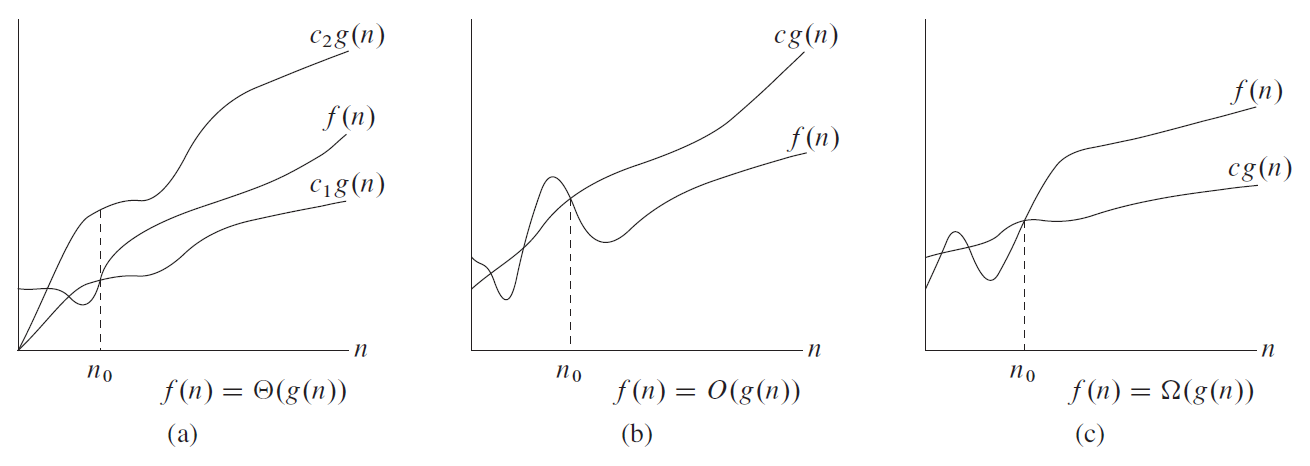
\includegraphics[width=\linewidth]{figuras/big-o}
  \caption{Interpretación gráfica de la notación asintótica. La notación \(f=O(g)\) implica que \(g\) es una cota superior para \(f\); esto es, \(g\) crece más rápido que \(f\) a partir de cierto valor de \(n\).}
\end{marginfigure}

\begin{marginfigure}
  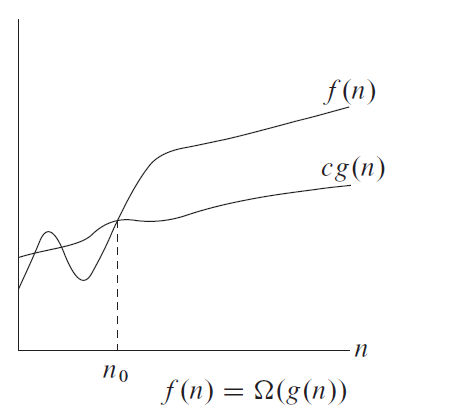
\includegraphics[width=\linewidth]{figuras/big-omega}
  \caption{La notación \(f=\Omega(g)\) implica que \(g\) es una cota inferior para \(f\); esto es, \(g\) crece más lento que \(f\) a partir de cierto valor de \(n\).}
\end{marginfigure}

\begin{marginfigure}
  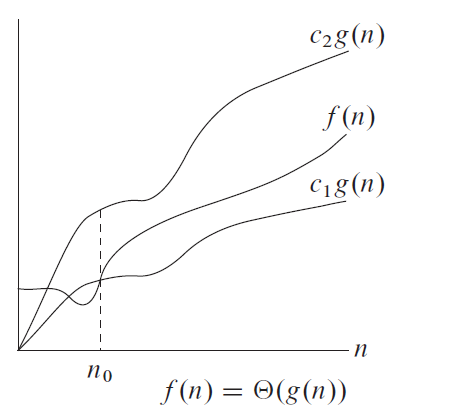
\includegraphics[width=\linewidth]{figuras/big-theta}
  \caption{La notación \(f=\Theta(g)\) implica que \(g\) acota a \(f\) por arriba y por abajo.}
\end{marginfigure}

Sea \(n\in\mathbb{N}\) y sean \(f:\mathbb{N}\to\mathbb{R}\) y \(g:\mathbb{N}\to\mathbb{R}\) dos funciones \textbf{asintóticamente no-negativas}; esto es, siempre se tiene que \(f(n)\geq 0\) y \(g(n)\geq 0\) a partir de algún valor determinado de \(n\). 

\begin{defn}[\textbf{O-grande}]
  Denotado como \(O(g)\), es el conjunto de todas aquellas funciones \(f\) para las cuales existen dos constantes, \(c\in\mathbb{R}^+\) y \(n_0\in\mathbb{N}\), tales que \(0\leq f(n)\leq cg(n)\) para toda \(n\leq n_0\).
\end{defn}

\begin{defn}[\(\boldsymbol{\Omega}\)\textbf{-grande}]
  Denotado como \(\Omega(g)\), es el conjunto de todas aquellas funciones para las cuales existen dos constantes, \(c\) y \(n_0\), tales que \(0\leq cg(n)\leq f(n)\) para toda \(n\geq n_0\).
\end{defn}

\begin{defn}[\(\boldsymbol{\Theta}\)\textbf{-grande}]
  Denotado como \(\Theta(g)\), es el conjunto de todas aquellas funciones para las cuales existen tres constantes, \(c_1,c_2\in\mathbb{R}^+\) y \(n_0\), tales que \(0\leq c_1 g(n)\leq f(n)\leq c_2 g(n)\) para toda \(n\geq n_0\).
\end{defn}

\begin{prop}
  Se tiene q. \(f=\Theta(g)\) si y solo si \(f=O(g)\) y \(f=\Omega(g)\).
\end{prop}

\begin{defn}[\textbf{o-chica}]
  Denotado como \(o(g)\), es el conjunto de todas aquellas funciones \(f\) para las cuales se cumple que, para toda constante \(c\), existe una constante \(n_0\) tal que \(0\leq f(n)<cg(n)\) para toda \(n\leq n_0\).
\end{defn}

\begin{defn}[\(\boldsymbol{\omega}\)\textbf{-chica}]
  Denotado como \(\omega(g)\), es el conjunto de todas aquellas funciones \(f\) para las cuales se cumple que, para toda constante \(c\), existe una constante \(n_0\) tal que \(0\leq cg(n)<f(n)\) para toda \(n\geq n_0\).
\end{defn}

\begin{prop}
  Si \(f=o(g)\), entonces \(f=O(g)\).
\end{prop}

\begin{prop}
  Si \(f=\omega(g)\), entonces \(f=\Omega(g)\).
\end{prop}

\begin{prop}
  Se tiene que
  \[
    \text{si }\lim_{n\to\infty}\dfrac{f(n)}{g(n)}=\begin{cases}
    0 & \text{entonces }f=o(g)\\
    \infty & \text{entonces }f=\omega(g)\\
    1 & \text{entonces }f=\Theta(g).
    \end{cases}
  \]
\end{prop}

\newpage
\section{Comparación de funciones por medio de la notación asintótica}

La notación asintótica se puede utilizar para comparar dos funciones y decidir cuál crece más rápido.

\begin{table}
  \label{tab:func-comp}
  \caption{Operaciones de comparación de los números reales y su funcionamiento análogo en la notación asintótica.}
  \centering
  \begin{tabular}{cc}
    \toprule 
      Números reales & Notación asintótica\tabularnewline
    \midrule
      \(a\leq b\) & \(f=O(g)\)\tabularnewline
      \(a\ge b\) & \(f=\Omega(g)\)\tabularnewline
      \(a=b\) & \(f=\Theta(g)\)\tabularnewline
      \(a<b\) & \(f=o(g)\)\tabularnewline
      \(a>b\) & \(f=\omega(g)\)\tabularnewline
    \bottomrule
  \end{tabular}
\end{table}

\paragraph{Transitividad} 
  Sea \(h:\mathbb{N}\to\mathbb{R}\) una función asintóticamente positiva.
  \begin{itemize}
    \item Si \(f=O(g)\) y \(g=O(h)\), entonces \(f=O(h)\).
    \item Si \(f=\Omega(g)\) y \(g=\Omega(h)\), entonces \(f=\Omega(h)\).
    \item Si \(f=\Theta(g)\) y \(g=\Theta(h)\), entonces \(f=\Theta(h)\).
    \item Si \(f=o(g)\) y \(g=o(h)\), entonces \(f=o(h)\).
    \item Si \(f=\omega(g)\) y \(g=\omega(h)\), entonces \(f=\omega(h)\).
  \end{itemize}

\paragraph{Reflexividad} 
  Se tiene que \(f=\Theta(f)\), \(f=O(f)\) y \(f=\Omega(f)\). 
  Esto se cumple porque \(f(n)=f(n)\) para toda \(n\).

\paragraph{Simetría y simetría traspuesta}
  \begin{itemize}
    \item \(f=\Theta(g)\) si y sólo si \(g=\Theta(f)\)
    \item \(f=O(g)\) si y sólo si \(g=\Omega(f)\).
    \item \(f=o(g)\) si y sólo si \(g=\omega(f)\).
  \end{itemize}

\paragraph{Carencia de tricotomía} 
  La tricotomía es la propiedad de los números reales donde, dados dos números, \(a\) y \(b\), siempre se cumple necesariamente una de las sig. posibilidades: \(a<b\), \(a=b\) o \(a>b\).
  Puede llegar a ocurrir que no se cumple que \(f=O(g)\) ni que \(f=\Omega(g)\).
  P. ej., el comportamiento asintótico de las funciones \(f(n)=n\) y \(g(n)=n^{1+\sin{n}}\) no se puede comparar porque el exponente \(1+\sin{n}\) oscila entre 0 y 2, tomando todos los valores intermedios y, como consecuencia, ninguna función consistentemente acota a la otra.

\marginnote[-14\baselineskip]{%
  Cabe mencionar que, dado que \(\Theta\)-grande posee las propiedades de reflexividad, transitividad y simetría, este conjunto es, de hecho, una \textbf{relación de equivalencia}.
}

\newpage
\section{Ordenes de crecimiento comúnes}

Listados de aquél que crece más lento al que crece más rápido.

\begin{enumerate}
  \begin{multicols}{2}
    \item \emph{Constantes}: \(O(1)\)
    \item \emph{Logarítmicos}: \(O(\log n)\)
    \item \emph{Radicales}: \(O(\sqrt{n})\)
    \item \emph{Lineales}: \(O(n)\)
    \item \emph{Súper lineales}: \(O(n\log n)\)
    \item \emph{Cuadráticos}: \(O(n^{2})\)
    \item \emph{Cúbicos}: \(O(n^{3})\)
    \item \emph{Exponenciales}: \(O(2^{n})\)
    \item \emph{Factoriales}: \(O(n!)\)
  \end{multicols}
\end{enumerate}

No se debe confiar ciegamente en la lista anterior, ya que la notación asintótica puede ocultar constantes muy grandes y dejar una impresión equivocada del orden de crecimiento de una función comparada con otra.
P. ej., \(f(n)=10^{100}n=O(n)\) y \(g(n)=10n\cdot\log n=O(n\log n)\). 
A pesar de que la notación asintótica indica que \(g\) crece más rápido que \(f\), en realidad se trata de lo opuesto porque la constante \(10^{100}\) supera por mucho el orden de crecimiento de \(g\)

\section{Operaciones aritméticas con la notación asintótica}

\paragraph{Adición}
  \[
  \begin{aligned}
      O(f)+O(g) &= O(\max\{f,g\})\\
      \Omega(f)+\Omega(g) &= \Omega(\max\{f,g\})\\
      \Theta(f)+\Theta(g) &= \Theta(\max\{f,g\})
  \end{aligned}
  \qquad
  \begin{aligned}
      o(f)+o(g) &= o(\max\{f,g\})\\
      \omega(f)+\omega(g) &= \omega(\max\{f,g\})
  \end{aligned}
  \]

\paragraph{Multiplicación}
  \[
  \begin{aligned}
      O(cf) &= O(f)\\
      \Omega(cf) &= \Omega(f)\\
      \Theta(cf) &= \Theta(f)
  \end{aligned}
  \qquad
  \begin{aligned}
      o(cf) &= o(f)\\
      \omega(cf) &= \omega(f)
  \end{aligned}
  \]

  \[
  \begin{aligned}
      O(f)\cdot O(g) &= O(f\cdot g)\\
      \Omega(f)\cdot\Omega(g) &= \Omega(f\cdot g)\\
      \Theta(f)\cdot\Theta(g) &= \Theta(f\cdot g)
  \end{aligned}
  \qquad
  \begin{aligned}
      o(f)\cdot o(g) &= o(f\cdot g)\\
      \omega(f)\cdot\omega(g) &= \omega(f\cdot g)
  \end{aligned}
  \]

\marginnote[-2\baselineskip]{%
  \textbf{Literatura consultada}: \textcite{cormen_2009}, pp. 43-52; \textcite{skiena_2012} pp. 34-41.
}

    \chapter{Métodos para resolver recurrencias}

\section{El método del árbol recursivo}

El método del árbol recursivo es un método gráfico e informal para resolver recurrencias y consiste en dibujar un árbol donde cada nodo representa el tiempo requerido para resolver un subproblema.
Al sumar el valor de todos los nodos del árbol, se puede obtener la solución de la recurrencia.
Antes de estudiar el método en sí, es importante recordar algunos conceptos sobre árboles.

Sea \(k\in\mathbb{N}\), un \textbf{árbol} \(\boldsymbol{k}\)\textbf{-ario} es un árbol enraizado donde cada nodo tiene a lo más \(k\) hijos. 
Un árbol \(k\)-ario \textbf{lleno} es aquél donde cada nodo es una hoja o tiene exactamente \(k\) hijos. 
La \textbf{profundidad} de un nodo es la distancia más corta entre dicho nodo y la raíz. 
Por definición, la raíz tiene una profundidad de 0.
Un árbol \(k\)-ario \textbf{completo} es un árbol lleno donde todas las hojas tienen la misma profundidad.
En un árbol \(k\)-ario completo, el número de nodos a profundidad \(d\) está dado por \(k^d\).
La \textbf{altura} de un árbol es la profundidad más grande de todos los nodos.
Así, la altura de un árbol \(k\)-ario completo de \(n\) hojas está dado por \(\log_k{n}\).
El número de nodos internos en un árbol \(k\)-ario completo de altura \(h\) está dado por
\[
  1+k+k^2+\dots+k^{h-1} = 
  \sum_{d=0}^{h-1}k^d =
  \sum_{d=1}^{h}k^d =
  \dfrac{k^h-1}{k-1}.
\]

\newpage
El método del árbol recursivo consta de los sig. pasos:

\begin{enumerate}
  \item Se dibuja el árbol recursivo de la recurrencia cumpliendo con las sig. características:
  \begin{itemize}
    \item La raíz contiene la expresión \(f(n)\) que representa el tiempo de ejecución requerido por la división y/o la combinación.
    \item Cada nodo interno contiene la expresión \(f(n_i)\), donde \(n_i<n\) es el tamaño del subproblema \(i\).
    \item Cada hoja contiene el tiempo de ejecución requerido por el caso base, que casi siempre es \(\Theta(1)\).
    \item Cada nodo interno tiene una cantidad de hijos equivalente al número de subproblemas en que se divide la entrada de cada llamada recursiva.
  \end{itemize}
  \item Se calcula la altura del árbol; esto es, la ruta más larga que sigue el algoritmo en el árbol para llegar al caso base.
  \item Se calcula la cantidad de hojas; esto es, el número de nodos en el nivel más profundo.
  \item Se suman los valores de todos los nodos por cada nivel.
  \item Se suman los resultados de todos los niveles, obtenidos en el paso anterior.
  \item Se resuelve la expresión resultante. %para obtener la forma cerrada.
\end{enumerate}

\begin{figure*}[t]
  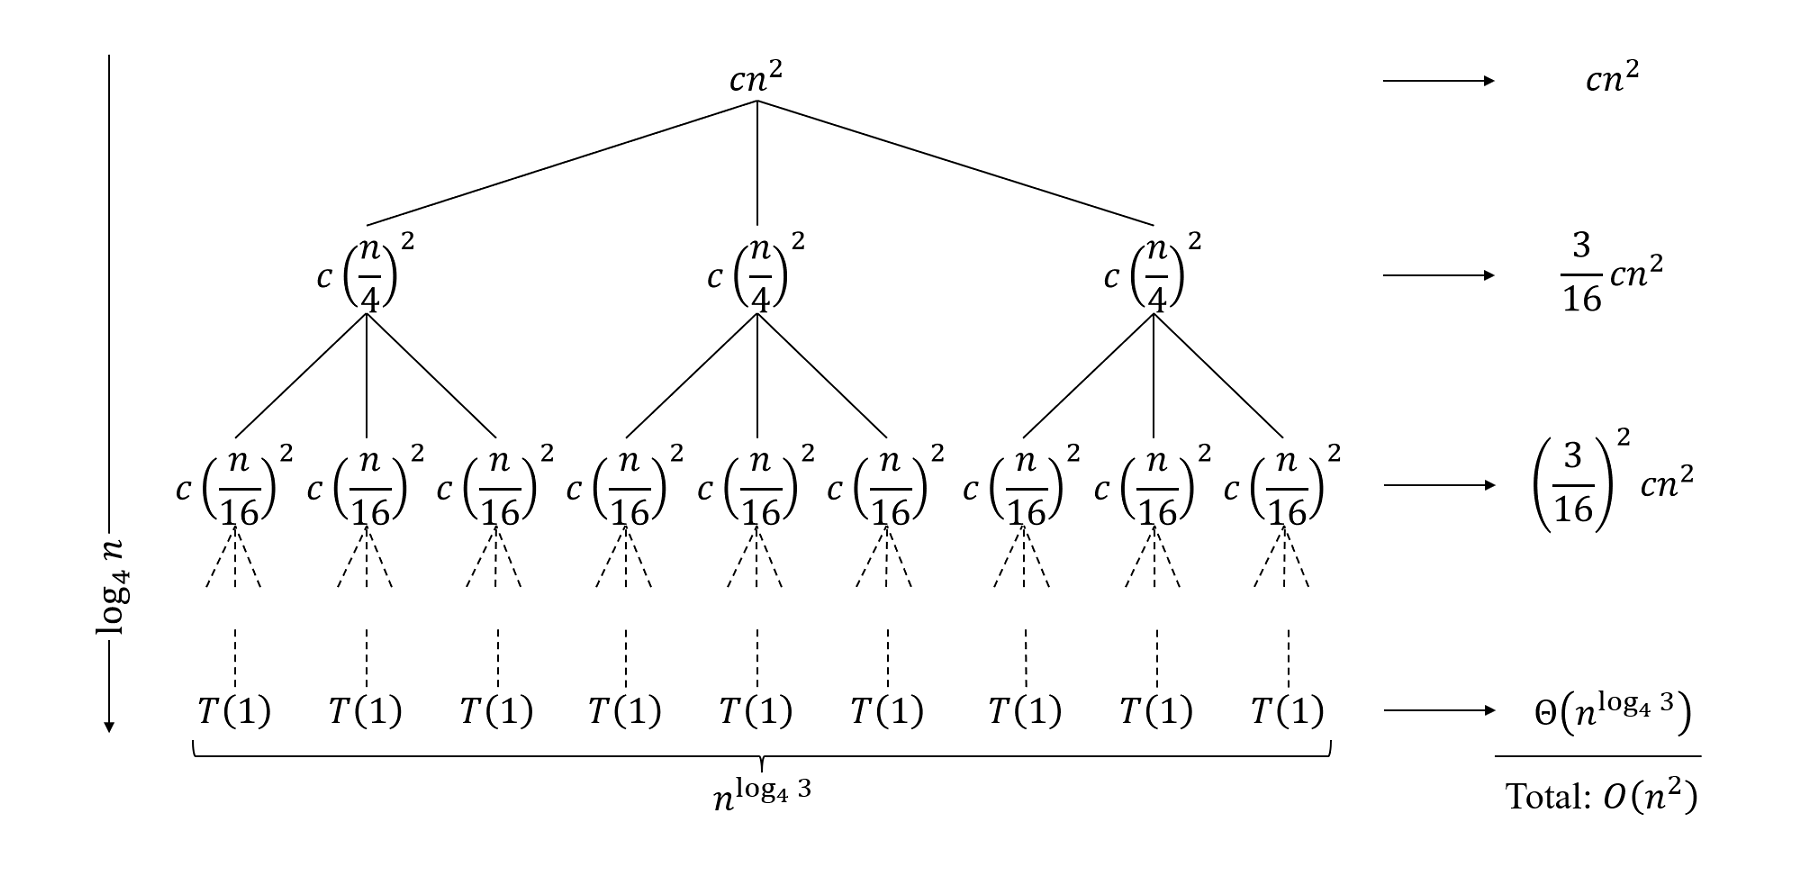
\includegraphics[width=1\textwidth]{figuras/recursion-tree.png}
  \caption{Usando el método del árbol recursivo para resolver la recurrencia \(T(n)=3T(n/4)+cn^{2}\).}
  \label{fig:recursion_tree}
\end{figure*}

\newpage

\begin{expl}
  Considérese la recurrencia \(T(n)=3T(n/4)+cn^2\). 
  Se debe dibujar el árbol recursivo, el cual se muestra en la Figura \ref{fig:recursion_tree}.
  Después, se debe calcular la altura del árbol. 
  Dado que el valor de \(n\) se reduce en un factor de \(1/4\) en cada nivel, la altura es el número de niveles que deben de recorrerse hasta llegar a 1. Así, la altura \(h\) puede calcularse como
  \[
    \begin{aligned}
      \left(\dfrac{1}{4}\right)^h\cdot n &= 1 \\
      \dfrac{1}{4^h}\cdot n &= 1 \\
      n &= 4^h \\
      \log_4{n} &= h.
    \end{aligned}
  \]
  
  Luego, se debe calcular el número de hojas.
  Dado que cada nodo tiene exactamente 3 hijos, el número de hojas está dado por
  \[
    3^h = 3^{\log_4{n}} = n^{\log_4{3}}.
  \]
  
  El siguiente paso es calcular el tiempo total de cada nivel.
  En la Figura \ref{fig:recursion_tree}, se observa que de dicha suma surge un patrón que se repite en función de \(cn^2\).
  En cuanto a la suma del último nivel, dado que el tiempo requerido por el caso base está dado por \(T(1)=\Theta(1)\), dicha suma es igual al número de hojas, que ya se calculó.
  
  Por último, se suman los tiempos de todos los niveles, lo que resulta en la sig. expresión:
  
  \begin{align*}
    T(n)&=\sum_{i=0}^{\log_{4}n-1}\left(\dfrac{3}{16}\right)^{i}\cdot cn^{2}+\Theta(n^{\log_{4}3}) \\
    &<\sum_{i=0}^{\infty}\left(\dfrac{3}{16}\right)^{i}\cdot cn^{2}+\Theta(n^{\log_{4}3}) \\
    &=\dfrac{1}{1-3/16}\cdot cn^{2}+\Theta(n^{\log_{4}3}) \\
    &=\dfrac{16}{13}\cdot cn^{2}+\Theta(n^{\log_{4}3}) \\
    &=O(n^{2})+O(n^{\log_{4}3}) \\
    &=O(n^{2}).
  \end{align*}
	\exend
\end{expl}
\newpage



\section{El método de sustitución}

El método de sustitución es un método formal que consiste en resolver una recurrencia utilizando inducción matemática. 
Específicamente, este método consta de los sig. pasos:
\begin{enumerate}
  \item Se propone una cota asintótica como la solución tentativa de la recurrencia.
  \item Se utiliza inducción para demostrar que la recurrencia cumple con la cota propuesta y para encontrar las constantes de dicha cota.
\end{enumerate}
Este método se puede utilizar para calcular tanto una cota superior como una inferior.

\paragraph{Para proponer una buena solución tentativa.}{%
  Se puede utilizar el método del árbol recursivo para obtener una solución tentativa.
  Después, se puede usar el método de sustitución para demostrar que dicha solución es correcta o para ajustar la cota en caso de que no lo sea.
  Otra alternativa es que, si la recurrencia tiene una forma similar a alguna otra cuya solución ya se conoce, se puede proponer esa solución como la solución tentativa.
  Como último recurso, se pueden proponer dos cotas holgadas, una inferior y  una superior, y ajustarlas gradualmente hasta que converjan en la solución correcta. 
}
\paragraph{Diferencias con la inducción matemática.}{%
  El caso base se demuestra hasta el final y no al principio de la demostración.
  La hipótesis inductiva consiste en suponer que la cota se cumple para cualquier subproblema, \(T(n_i)\), donde \(n_i<n\). 
  El paso inductivo consiste en sustituir \(T(n_i)\) (en la recurrencia original) por la forma exacta de la cota propuesta en la hipótesis inductiva. 
  Este paso da origen al nombre del método.
}
\paragraph{Cuidado con la notación asintótica.} {%
  El objetivo del método de sustitución es demostrar algebraicamente que 
  la cota propuesta se cumple de \emph{forma exacta}.
  Es incorrecto aplicar la notación asintótica en el paso inductivo para deshacerse de constantes o términos problemáticos.
}

\newpage
\begin{expl}
  \label{ex:recurrence_substitution}
  Considérese la recurrencia \(T(n)=2T(\lfloor n/2 \rfloor)+n\) y supóngase que se propone \(O(n\lg{n})\) como la solución tentativa. 
  Entonces, se busca demostrar que \(T(n)\leq cn\lg{n}\) para alguna constante \(c>0\).
  \begin{description}
    \item[Hipótesis inductiva] Supóngase que \(T(\lfloor n/2\rfloor)\leq c\lfloor n/2\rfloor\lg\lfloor n/2\rfloor\).
    \item[Paso inductivo] Sustituyendo la hipótesis inductiva en la recurrencia original, se tiene:
    \begin{align*}
      T(n) &\leq2c\lfloor n/2\rfloor\lg\lfloor n/2\rfloor+n \\
      &\leq cn\lg(n/2)+n \\
      &=cn\lg n-cn\lg2+n \\
      &=cn\lg{n}-cn+n \\
      &\leq cn\lg n.
    \end{align*}
    Aparentemente, la solución propuesta es la correcta (para toda \(c\geq 1\)). 
    Sin embargo, hace falta demostrar que esta solución también se cumple para la condición de paro de la recurrencia. 
    Esto debe demuestrarse por construcción; esto es, se debe encontrar un valor para \(c\) que satisfaga la cota en la condición de paro. 
    A continuación, se muestra cómo esto puede llevar a ciertos problemas. 
    \item[Caso base] Supóngase que \(T(1)=1\). 
    Aplicando la cota propuesta a la condición de paro, se tiene que \(T(1)\leq cn\lg n=c\lg{1}=0\), lo que contradice que \(T(1)=1\). 
    Por lo tanto, la solución propuesta falla en el caso base. 
    Sin embargo, hay que recordar que la definición de la notación asintótica requiere que la cota se cumpla únicamente para un valor de \(n\) mayor que algún umbral \(n_{0}\) que \emph{uno es libre de elegir a voluntad}. 
    Esto quiere decir que no es obligatorio utilizar la condición de paro de la recurrencia como el caso base de la inducción. 
    Para este ejemplo, obsérvese que \(T(\lfloor2/2\rfloor)=T(\lfloor3/2\rfloor)=T(1)\), por lo que se puede utilizar \(T(2)\) y \(T(3)\) como el caso base. 
    Esto es equivalente a elegir \(n_0=2\).
    Aplicando la hipótesis inductiva al nuevo caso base, se tiene:
    \begin{align*}
      T(2) & \leq 2c\lg2 & T(3) & \leq 3c\lg3 \\
      2T(\lfloor 2/2 \rfloor) + 2 & \leq 2c & 2T(\lfloor 3/2 \rfloor) + 3 & \leq 3c(1.585) \\
      2T(1) + 2 & \leq2c & 2T(1) + 3 & \leq 3c(1.585) \\
      4 & \leq 2c & 5 & \leq 3c(1.585) \\
      2 & \leq c, & \dfrac{5}{4.755} & \leq c.
    \end{align*}
    Por lo tanto, queda demostrado que \(T(n)\leq cn\lg{n}\) para toda \(c\geq 2\). \exend
  \end{description}
\end{expl}

\newpage
\begin{expl}
    Considérese ahora la recurrencia \(T(n)=T(\lfloor n/2\rfloor)+T(\lceil n/2\rceil)+1\) y supóngase que se propone \(O(n)\) como la solución tentativa. 
    Se busca demostrar que \(T(n)\leq cn\) para alguna \(c>0\).
    \begin{description}
      \item[Hipótesis inductiva] Supóngase que \(T(\lfloor n/2\rfloor)\leq c\lfloor n/2\rfloor\) y que \(T(\lceil n/2\rceil)\leq c\lceil n/2\rceil\).
      \item[Paso inductivo] Sustituyendo la hipótesis inductiva en la recurrencia original, se tiene: \(T(n) \leq c\lfloor n/2 \rfloor + 1 = cn + 1\).
      Esto sugiere que la solución propuesta no es correcta.
      En este ejemplo, se ve que el término \(+1\) impide que la igualdad se cumpla de forma exacta.
      En lugar de proponer una cota más holgada, se propone une nueva hipótesis inductiva.
      \item[Nueva H.I.] Supóngase que \(T(\lfloor n/2\rfloor)\leq c\lfloor n/2\rfloor-d\) y que \(T(\lceil n/2\rceil)\leq c\lceil n/2\rceil-d\), donde \(d\in\mathbb{R}\) tal que \(d\geq 0\).
      \item[Paso inductivo] Sustituyendo la hipótesis inductiva en la recurrencia original, se tiene lo sig.:
      \begin{align*}
        T(n) &\leq c\lfloor n/2\rfloor-d+c\lceil n/2\rceil-d+1\\
        &=cn-2d+1\\
        &\leq cn-d.
      \end{align*}
      Esto se cumple para toda \(d\geq 1\). 
      Ahora solo queda demostrar que la cota se cumple para la condición de paro.
      \item[Caso base] Obsérvese que \(n=2\) es el valor más pequeño que resulta en \(T(1)\), tanto para \(T(\lfloor n/2 \rfloor)\) como para \(T(\lceil n/2 \rceil)\). 
      Aplicando la hipótesis inductiva a estos términos, se tiene que:
      \begin{align*}
        T(2) &\leq 2c-d\\
        T(\lfloor 2/2 \rfloor) + T(\lceil 2/2 \rceil) + 1 &\leq 2c-d \\
        2T(1) + 1 &\leq 2c - d \\
        \dfrac{2T(1)+1+d}{2} &\leq c \\
        T(1) + \dfrac{1+d}{2} &\leq c.
      \end{align*}
      \exend
    \end{description}
\end{expl}


\newpage
\section{El Teorema Maestro}

\begin{thm}[\textbf{Teorema Maestro}]
  Sean \(a,b,n\in\mathbb{N}\), donde \(a\) y \(b\) son constantes y \(b>1\), sea \(f:\mathbb{N}\to\mathbb{N}\) una función asintóticamente positiva y sea \(c=\log_{b}a\). 
  La recurrencia \(T(n)=aT(n/b)+f(n)\) puede resolverse aplicando uno de los sig. casos:
  \begin{enumerate}
    \item Si \(f(n)=O(n^{c-\varepsilon})\) para alguna constante real $\varepsilon>0$, entonces \(T(n)=\Theta(n^{c})\).
    \item Si \(f(n)=\Theta(n^c)\), entonces \(T(n)=\Theta(n^{c}\log{n})\).
    \item Si \(f(n)=\Omega(n^{c+\varepsilon})\) y si, además, \(af(n/b)\leq kf(n)\) para alguna constante real \(k<1\) y para todo valor de \(n\) mayor que algún umbral, entonces \(T=\Theta(f)\).
  \end{enumerate}
\end{thm}

\begin{rem}
  En el Teorema Maestro, el término \(n/b\) de la recurrencia \(T(n)\) también puede interpretarse como \(\lceil n/b\rceil\) o \(\lfloor n/b\rfloor\).
\end{rem}

El Torema Maestro solo puede aplicarse a recurrencias que dividen el problema en \(a\) subproblemas \emph{del mismo tamaño}, y donde, en cada subproblema, el tamaño de la entrada se reduce en un factor de \(1/b\).
La función \(f(n)\) representa el tiempo de ejecución para dividir el problema y/o combinar las soluciones parciales de los subproblemas.
La función \(n^c\) representa el número de hojas en el árbol recursivo de la recurrencia.

Intuitivamente, el Teorema Maestro indica que, comparando \(n^c\) con \(f(n)\), la función que crece más rápido es la solución de la recurrencia.
\begin{itemize}
  \item \textit{Caso 1}: \(n^c\) crece más rápido; esto es, el tiempo requerido para resolver cada subproblema eventualmente supera el tiempo requerido por la división y/o combinación.
  \item \textit{Caso 2}: ambas funciones, \(f(n)\) y \(n^c\), tienen la misma tasa de crecimiento.
  En este caso, la solución es el orden de crecimiento de estas funciones, multiplicado por un factor logarítmico que representa la altura del árbol recursivo (ya que cada nivel del árbol requiere el mismo tiempo de ejecución).
  \item \textit{Caso 3}: \(f(n)\) crece más rápido que \(n^c\). 
  Si \(f(n)\), además, cumple con la \textbf{condición de regularidad}, entonces esta función es la solución de la recurrencia.
\end{itemize}

\section{Notas bibliográficas}

En el libro de \textcite{cormen_2009}, págs. 97-106, se proporciona la demostración del Teorema Maestro.
Además, en las págs. 112-113, se describe el \textbf{método de Akra-Bazzi} \citep{akra_1998,leighton_1996}, que se utiliza para resolver recurrencias donde el problema se divide en subproblemas que difieren mucho de tamaño.
Este método trabaja con variables contínuas.
Por otro lado, \textcite{drmota_2013} presentan una especialización del método de Akra-Bazzi que trabaja con variables discretas. 

\marginnote[-1\baselineskip]{%
  \textbf{Literatura consultada}: \textcite{cormen_2009} pp. 65-67, 83-97.
}

  
  \part{Anexos}
    \chapter{La potencia}

Sea \(x\in\mathbb{R}\) distinto de cero y denominado \emph{base} y sea \(n\in\mathbb{N}\) denominado \emph{exponente}. 
La \emph{n-ésima potencia} de \(x\), denotada como \(x^n\), es el producto de \(n\) bases \(x\); esto es, \(x^n\triangleq x\cdot x\cdot\dots(n\text{ veces})\).

\section{Leyes de los exponentes}

Sean \(x,y\in\mathbb{R}\) distintos de cero y sean \(m,n\in\mathbb{N}\).
Se tienen las sig. identidades:
\begin{enumerate}
  \begin{multicols}{3}
    \item \(x^{0}\triangleq1\)
    \item \(x^{1}\triangleq x\)
    \item \(x^{-1}\triangleq1/x\)
    \item \(x^{m/n}\triangleq\sqrt[n]{x^{m}}\)
    \item \(x^{m}x^{n}=x^{m+n}\)
    \item \(x^{m}/x^{n}=x^{m-n}\)
    \item \((x^{m})^{n}=x^{mn}\)
    \item \((xy)^{n}=x^{n}y^{n}\)
    \item \((x/y)^{n}=x^{n}/y^{n}\)
  \end{multicols}
\end{enumerate}

Las identidades anteriores se justifican de las sig. manipulaciones algebraicas:

\begin{flalign}\tag{5}
  x^mx^n &= x\cdot x\cdot\dots (m\text{ veces})\cdot x\cdot x\dots (n\text{ veces}) &&\\
  &= x^{m+n}\nonumber
\end{flalign}

\begin{flalign}\tag{6}
  \text{\textit{Caso 1}} &: \text{ Si }m>n\text{, entonces} \nonumber&&\\
  x^m/x^n &= \dfrac{x\cdot x\cdot\dots (m\text{ veces})}{x\cdot x\cdot\dots (n\text{ veces})} \nonumber&&\\
  &= 1\cdot 1\cdot\dots(n\text{ veces})\cdot x\cdot x\cdot\dots(m-n\text{ veces}) \nonumber&&\\
  &=x^{m-n} \nonumber&&\\
  \text{\textit{Caso 2}} &: \text{ Si }m=n\text{, entonces} \nonumber&&\\
  x^m/x^n &=1\cdot 1\cdot\dots (m=n\text{ veces}) \nonumber&&\\
  &=x^0 \nonumber&&\\
  &=x^{m-n}\nonumber&&\\
  \text{\textit{Caso 3}} &: \text{ Si }m<n\text{, entonces} \nonumber&&\\
  x^m/x^n &=1\cdot 1\cdot\dots(m\text{ veces})\cdot 1/x\cdot 1/x\cdot\dots(n-m\text{ veces}) \nonumber&&\\
  &=1/x^{n-m} \nonumber&&\\
  &=x^{m-n} \nonumber
\end{flalign}

\begin{flalign}\tag{7}
  (x^m)^n &= [x\cdot x\cdot\dots (m\text{ veces})]\cdot[x\cdot x\cdot\dots (m\text{ veces})]\dots[n\text{ veces}] &&\\
  &= x^{mn}\nonumber
\end{flalign}

\begin{flalign}\tag{8}
  (xy)^n &= xy\cdot xy\cdot\dots (n\text{ veces}) &&\\
  &= x\cdot x\cdot\dots (n\text{ veces})\cdot y\cdot y\cdot\dots (n\text{ veces}) \nonumber&&\\
  &= x^ny^n\nonumber
\end{flalign}

\begin{flalign}\tag{9}
  (x/y)^n &= \dfrac{x}{y}\cdot\dfrac{x}{y}\cdot\dots (n\text{ veces}) &&\\
  &= x^n/y^n\nonumber
\end{flalign}

    \chapter{El logaritmo}

Sea \(x\in\mathbb{R}\) mayor a cero y denominado \emph{argumento} y sea \(b\in\mathbb{R}\) distinto de 1 y denominado \emph{base}.
El \emph{logaritmo} de \(x\) con respecto a \(b\), denotado como \(\log_{b}x\), es la potencia a la que hay que elevar \(b\) para obtener \(x\) como resultado; esto es, \(y=\log_{b}x\) si y sólo si \(b^{y}=x\), donde \(y\in\mathbb{R}\).

\begin{table}[h]
  \caption{Diferentes tipos de logaritmos, su base y su notación correspondiente.}
  \begin{center}
    \begin{tabular}{ccc}
      \toprule
      Tipo de logaritmo & Base & Notación \\
      \midrule
      Decimal & 10 & \(\log{x}\) \\
      Natural & \(e\) & \(\ln{x}\) \\
      Binario & 2 & \(\lg{x}\) \\
      \bottomrule
    \end{tabular}
  \end{center}
\end{table}

\begin{prop}
  La base de un logaritmo no puede ser 0 ni 1.
\end{prop}
  
Debido a que \(0^x=0\) para toda \(x>0\) y debido a que \(1^x=1\) para toda \(x\), los logaritmos con base 0 y 1 no tienen una solución definida.

\begin{prop}
  La base de un logaritmo no puede ser negativa.
\end{prop}

De lo contrario, dependiendo del argumento del logaritmo, la solución podría ser un número complejo.

\begin{prop}
  El argumento de un logaritmo no puede ser negativo.
\end{prop}

Debido a que todo número positivo elevado a cualquier potencia siempre resulta en un número positivo, el logaritmo (con base positiva) de un número negativo no tendría solución.

\section{Leyes de los logaritmos}

Sean \(b,v,x,y\in\mathbb{R}\), donde los valores \(x\) y \(y\) son mayores a cero y los valores \(b\) y \(v\) son distintos de 1. Se tienen las sig. identidades:

\marginnote[1\baselineskip]{La identidad 7 se conoce como la ley de cambio de base. Esta ley implica que \(\log_v{x}=\log_v{b}\cdot\log_b{x}\); esto es, para cambiar la base de un logaritmo, basta con multiplicarlo por un factor constante. Debido a esto, no importa la base de un logaritmo, su comportamiento asintótico siempre será el mismo y es por esta razón que la base del logaritmo suele omitirse al utilizar la notación asintótica.}

\begin{enumerate}
  \begin{multicols}{2}
    \item \(\log_b{1}=0\)
    \item \(\log_b{b}=1\)
    \item \(\log_b(xy)=\log_b{x}+\log_b{y}\)
    \item \(\log_b(x/y)=\log_b{x}-\log_b{y}\)
    \item \(\log_bx^y=y\log_b{x}\)
    \item \(\log_b\sqrt[y]{x}=1/y\cdot\log_b{x}\)
    \item \(\log_b{x}=\log_v{x}/\log_v{b}\)
    \item \(\log_b{x}=1/\log_x{b}\), si \(x\neq 1\)
    \item \(x^{\log_b{y}}=y^{\log_b{x}}\)
  \end{multicols}
\end{enumerate}

Las identidades anteriores se justifican de las manipulaciones algebraicas que se presentan a continuación. Considérese que \(p,q\in\mathbb{R}\) tales que \(x=b^p\) y \(y=b^q\), lo que implica que \(p=\log_b{x}\) \& \(q=\log_b{y}\) (por la definición del logaritmo):
\begin{flalign}
  \text{Es consecuencia directa del hecho que } b^0=1\text{ para cualquier }b.
\end{flalign}
\begin{flalign}
  \text{Es consecuencia directa del hecho que } b^1=b\text{ para cualquier }b.
\end{flalign}
\begin{align}
  xy &= b^pb^q &&\\
  xy &= b^{p+q} \nonumber&&\\
  \log_b(xy) &= p+q \nonumber&&\\
  \log_b(xy) &= \log_b{x}+\log_b{y} \nonumber
\end{align}
\begin{align}
  x/y &= b^p/b^q &&\\
  x/y &= b^{p-q} \nonumber&&\\
  \log_b(x/y) &= p-q \nonumber&&\\
  \log_b(x/y) &= \log_b{x}-\log_b{y} \nonumber
\end{align}
\begin{align}
  x &= b^p &&\\
  x^y &= (b^p)^y \nonumber&&\\
  x^y &= b^{py} \nonumber&&\\
  \log_b{x^y} &= py \nonumber&&\\
  \log_b{x^y} &= y\log_b{x} \nonumber
\end{align}
\begin{align}
  x &= b^p &&\\
  \sqrt[y]{x} &= \sqrt[y]{b^p} \nonumber&&\\
  \sqrt[y]{x} &= b^{p/y} \nonumber&&\\
  \log_b \sqrt[y]{x} &= p/y \nonumber&&\\
  \log_b \sqrt[y]{x} &= 1/y\cdot \log_b{x} \nonumber
\end{align}
\begin{align}
  b^p &= x &\\
  \log_v{b^p} &= \log_v{x} \nonumber&&\\
  p\log_v{b} &= \log_v{x} \nonumber&&\\
  p &= \dfrac{\log_v{x}}{\log_v{b}} \nonumber&&\\
  \log_b{x} &= \log_v{x}/\log_v{b} \nonumber
\end{align}
\begin{align}
  \log_b{x} &= \dfrac{\log_v{x}}{\log_v{b}} &&\\
  \log_b{x} &= \dfrac{\log_x{x}}{\log_x{b}} \nonumber&&\\
  \log_b{x} &= \dfrac{1}{\log_x{b}} \nonumber
\end{align}
\begin{align}
  x^{\log_b{y}}=x^q=(b^p)^q=b^{pq}=(b^q)p=y^p=y^{\log_b{x}}
\end{align}

  
  \printbibliography[heading=bibintoc,title={Literatura consultada}]
\end{document}
